
\documentclass[11pt,a4paper,twoside]{article}

\usepackage[numbers, authoryear]{natbib}
\usepackage{url}
\usepackage{parskip}
\usepackage{graphicx}

\setlength{\oddsidemargin}{-0.4mm} % 25 mm left margin
\setlength{\evensidemargin}{\oddsidemargin}
\setlength{\textwidth}{160mm}      % 25 mm right margin
\setlength{\topmargin}{-5.4mm}     % 20 mm top margin
\setlength{\headheight}{5mm}
\setlength{\headsep}{5mm}
\setlength{\footskip}{10mm}
\setlength{\textheight}{237mm}     % 20 mm bottom margin
\setlength{\parindent}{12pt}
\begin{document}

\setcounter{page}{1}

\title{Implementing a Personal Container}
\author{Chris Elsmore}
%\date{} % do not add a date1
\date{October 2011}

\maketitle % optional

\begin{abstract}
This document explains the motivation behind setting up a personal container style data store, and the advantages such a container can provide. Online services are becoming more popular and more numerous, however with this growth comes greater scattering of personal data. We discuss using a Personal Container allows this data to be stored where the user chooses, in the cloud or on a computer at home, preventing data loss in the closure of an online service. This also allows a user to more closely allow or deny access to their data, along with letting third parties run algorithms on their personal container and return results without exposes the raw information. Using an implementation of the Personal Container paradigm called Locker, we can setup infrastructure internally, and use it to provide detailed information to a user based on their personal and sensitive data without exposing the raw data and compromising privacy. We show an example of this infrastructure by deploying it within the University as a pilot study, to identify the benefits both to employees who can use the container to store information, and the university that can request access to this information for survey's, and future decision making.
\end{abstract}

\newpage
% \tableofcontents % optional
%\section{Introduction}

\section{Motivation}

\subsection{Current Practice \& Limitations}
Online services and social networking websites have surged in popularity and now enjoy vast user bases - Facebook currently has 800 Million active users\cite{facebook:qr}, and Foursquare has acquired 100 Million Users in its 27 month lifetime\cite{foursquare:sd}. Sites also store a significant amount of user generated content - members upload 8 years worth of video using YouTube, 250 million photos to Facebook and generate over 200 million tweets on Twitter each day\cite{youtube:sa},\cite{twiter:st}.

The users who generate this data must trust that these sites will continue to exist to continue accessing this content. In the case of photo sharing sites the user most likely has copies of the images elsewhere, but does not have their own copy of the metadata generated after upload for example conversations regarding photos. Sites like Twitter and Foursquare by their nature don't generate any data locally, and all tweet and checkin data is stored remotely by the service. If these sites were to disappear, each user would not have a copy of their information without manually accessing, often using custom code using an API, a high barrier of entry for the non-technical user.

Even if the users are technically savvy and willing to write code, or trust 3rd party applications that access data on their behalf, users with a wide reaching digital footprint will require many different apps accessing many different API endpoints to reach their data, all with their own idiosyncratic behaviour within standards such as OAuth\footnote{More information available at \url{http://oauth.net/}}, used for authentication. Access to this data is further burdened by the use of certain 3rd party applications which in the case of Facebook have been known to have security and privacy concerns \cite{consumerist:sa} \cite{ZDnet:cs} \cite{wsj:sa} \cite{eff:sa}.

%Email daniel for cites?

%Users who generate this content and use these services 
%everyone has a digital footprint, with lots of data spread out over the internet.

%trust that these platforms will continue to exist,
%access to the data is A hard because its all over the place, and B often involves giving away a lot more access than you really want to.

\newpage
\section{Personal Containers}

\subsection{Description}
Personal Containers are designed to solve the problem of the fragmentation of user data throughout the social web, compute additional, higher resolution and more accurate personal data by combining multiple data sources, and facilitate tighter security around access to these data. They are basic data storage and access systems, and can range from simple databases of information on a single computer hosted by the user, to sophisticated systems that act as signposts, storing the location of all user data on multiple devices and services, and proxying requests to the relevant data sources.

%a container for all your online data - photos, tweets, status updates etc, and all the meta data too.

\subsection{Benefits}

Personal Containers provide a central access point to and allow autonomous collection of a users data from multiple sources, with data such as photos, tweets, status updates, checkins etc. Since the container provides direct access to multiple sources of data, it is able to generate far higher resolution data than using data from just one service- for example using geo-tagged tweets, photos and checkins along with Google Latitude\footnote{More information available at \url{http://google.com/latitude/}} data to provide highly accurate location information. It also allows faster and simpler access to multiple data, enable simple queries such as requesting all photos taken between two dates.

Personal Containers also ofter the possibility of increased security and data control. Personal data is by definition personal, and thus highly sensitive. The example above demonstrate the need to added security, when dealing with highly accurate and real-time location data for example. The personal container can use multiple factors to approve or deny requests based on traditional variables such as rate of access, and simple authentication, as well as time based restrictions such as validity windows where data access is only allowed for a certain time, and impose certain restrictions based on media type such as picture or location resolution.

The container can also allow results based on computation on personal container data to be accessed without allowing direct access to the data itself.

The data security befits are not only a matter of authentication, personal containers can act as sophisticated backup mechanisms of sensitive data, de-duplicating and federating throughout storage nodes such as personal computers at a users home or workplace, or instances running on cloud computing platforms such as Amazon's EC2\footnote{More information available at \url{http://aws.amazon.com/ec2/}}.

%allow fine grained control over access to said data, possibility to base it on recipient / time / number of accesses etc.
%allows for computation of external code without giving away access to the actual data, returns only the results.
%one place allows multiple data sources to be queried quickly.
%control over your own data - hosted in the cloud, or yourself.

\newpage
\section{Implementation}

\subsection{Architecture}
The Locker Project\footnote{More information available at \url{http://lockerproject.org/}} aims to construct a personal container suitable for hosting on a users general use computer, as well as adapting to a cloud based platform or a dedicated machine hosted personally. It is written in Javascript on the Node.js\footnote{More information available at \url{http://nodejs.org/}} platform on the backend, and standard HTML and Javascript on the web-based user interface. 

%what locker is - what its coded in and who is working on it.
%basic overall idea of how the individual bits work - web driven, locker core, collections, connectors, apps.

\subsection{Infrastructure}
Our deployment infrastructure involves multiple instances of the locker platform, installed on multiple virtual machines running a Linux OS with a secure proxy frontend. The locker codebase supports only single users with no authentication, so each instance is isolated within it's own virtual machine. A central Nginx\footnote{More information available at \url{http://nginx.org/}} server handles SSL encryption, authentication and acts as a proxy to direct to the correct instance based on the hostname requested internally to the host machine.

The deployment is hosted by the university cloud computing service, as an example of an institution hosting secure personal data storage, in return for access to said data in an open, and transparent way, identifying to the user exactly which data will be used, and for what purpose.
%Multiple lockers in VMs with a Nginx secure frontend. Hosted by the uni, for employees,

\newpage
\subsection{Advantages}


\begin{figure}[h]
  \begin{center}
    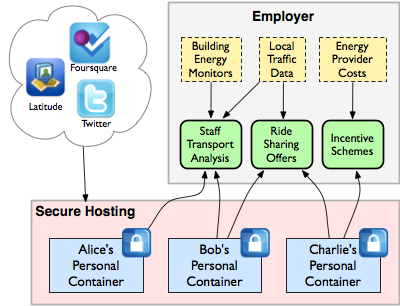
\includegraphics[scale=0.7]{PersConDataflow.png}
  \end{center}
  \caption{C-Aware Personal Container deployment layout.}
  \label{img-persConDia}
\end{figure}

As shown in figure \ref{img-persConDia}, using this system an employer can offer a range of schemes to it's employees, as well as using this data for it's own projects. For example the employer can use this data to fill out it's own transport survey questionnaires, gathering data on how it's employees travel to and from work, and use this to help decide weather a new car park is needed, or better cycle routes on its property.

It also enables the university to deliver more personal benefits to its users, for example knowing how much and when a user uses their energy can be used to provide a price comparison feature that shows exactly how much a users energy bill would be with different suppliers.
%allows employees to know their energy use whilst at work,
%allows uni to offer transport anaylsis, and give a comprehensive carbon footprint estimate
%Allows uni to offer schemes to employees such as car pooling.

\newpage
\bibliographystyle{abbrv}
\renewcommand{\bibname}{References} % changes default name Bibliography to References
\bibliography{LockerTechReport} % References file
%\addcontentsline{toc}{chapter}{References} %adds References to contents page

\end{document}